% Generated fragments require trusted human review before compilation.
% This binder never requests shell escape or runs external tools.
\documentclass[11pt]{article}
% Trusted shared apparatus. Requires LuaLaTeX; never use shell escape.
\usepackage{fontspec}
\defaultfontfeatures{Ligatures=TeX}
\IfFontExistsTF{Noto Serif}{\setmainfont{Noto Serif}}{%
  \IfFontExistsTF{DejaVu Serif}{\setmainfont{DejaVu Serif}}{%
    \IfFontExistsTF{Times New Roman}{\setmainfont{Times New Roman}}{%
      \PackageError{gelfand-binder}{No configured Cyrillic serif font installed}{Install Noto Serif or DejaVu Serif, or select an installed Cyrillic font.}%
    }%
  }%
}
\IfFontExistsTF{Noto Sans}{\setsansfont{Noto Sans}}{%
  \IfFontExistsTF{DejaVu Sans}{\setsansfont{DejaVu Sans}}{\setsansfont{Arial}}%
}
\IfFontExistsTF{Noto Sans Mono}{\setmonofont{Noto Sans Mono}}{%
  \IfFontExistsTF{DejaVu Sans Mono}{\setmonofont{DejaVu Sans Mono}}{\setmonofont{Courier New}}%
}
\usepackage[a4paper,margin=22mm]{geometry}
\usepackage{amsmath,amssymb,amsthm,mathtools}
\usepackage{xcolor}
\usepackage{tikz}
\usepackage{tikz-cd}
\usetikzlibrary{arrows.meta,positioning,calc}
\usepackage{hyperref}
\hypersetup{unicode=true,colorlinks=true,linkcolor=blue,pdftitle={Gelfand transcription binder}}
\newtheorem{theorem}{Theorem}
\newtheorem{lemma}{Lemma}
\newtheorem{proposition}{Proposition}
\newtheorem{corollary}{Corollary}
\theoremstyle{definition}
\newtheorem{definition}{Definition}
\newtheorem{example}{Example}
\theoremstyle{remark}
\newtheorem{remark}{Remark}
\setlength{\parindent}{0pt}
\setlength{\parskip}{0.55em}
\setlength{\emergencystretch}{3em}
\newcommand{\SourcePage}[2]{%
  \clearpage\phantomsection\label{#1:source-page}%
  \addcontentsline{toc}{subsection}{#1}%
  {\small\sffamily\color{blue!60!black}Source scan frame: #1; visible page/leaf label: #2}\par\medskip%
}
\newcommand{\Unclear}[3]{%
  \begingroup\color{orange!70!black}%
  [Unresolved reading #1/#2: #3]\endgroup%
}
\newcommand{\Incomplete}[3]{%
  \par\begingroup\color{red!65!black}\textbf{Incomplete #1/#2:} #3\endgroup\par%
}
\newcommand{\SourceFigure}[3]{%
  \par\begingroup\color{blue!60!black}\textbf{\hyperref[#1:source-page]{Source figure #1/#2}:} #3%
  \par\textit{Consult the authoritative scan at this locator.}\endgroup\par%
}



% Reader layout only. Original diplomatic text is retained verbatim.
\setlength{\parskip}{0.35em}
\setlength{\emergencystretch}{4em}
\renewcommand{\SourcePage}[2]{%
  \par\addvspace{1em}\phantomsection\label{#1:source-page}%
  \addcontentsline{toc}{subsection}{#1}%
  {\footnotesize\sffamily\color{blue!55!black}#1%
    \def\givenlabel{#2}\def\nolabel{unlabelled}%
    \ifx\givenlabel\nolabel\else\quad[номер в источнике: #2]\fi
  }\par\nobreak\smallskip%
}
\renewcommand{\Unclear}[3]{%
  \begingroup\color{orange!65!black}%
  \ifmmode\text{[неясно: #3]}\else[неясно: #3]\fi\endgroup%
}
\renewcommand{\Incomplete}[3]{%
  \par\begingroup\color{red!60!black}\textbf{Неразобранный фрагмент:} #3%
  \endgroup\par%
}
\renewcommand{\SourceFigure}[3]{%
  \par\begingroup\color{blue!55!black}\textbf{Рисунок:} #3%
  \par{\small\textit{Исходный рисунок: \hyperref[#1:source-page]{#1}, #2.}}%
  \endgroup\par%
}
\hypersetup{pdftitle={Семинар И. М. Гельфанда. Дипломатическая транскрипция},pdfauthor={},pdfsubject={Русское рабочее издание с отмеченными сомнительными чтениями}}

\usepackage[normalem]{ulem}
\usepackage{newunicodechar}
\usepackage{adjustbox}
\newfontfamily\SourceSymbolFont{Segoe UI Symbol}
\newfontfamily\SourceCJKFont{MS Gothic}
\let\DiplomaticMathUnderline\underline
\renewcommand{\underline}[1]{\ifmmode\DiplomaticMathUnderline{#1}\else\uline{#1}\fi}
\newunicodechar{→}{\ifmmode\text{{\SourceSymbolFont\char"2192}}\else{\SourceSymbolFont\char"2192}\fi}
\newunicodechar{⇒}{\ifmmode\text{{\SourceSymbolFont\char"21D2}}\else{\SourceSymbolFont\char"21D2}\fi}
\newunicodechar{∀}{\ifmmode\text{{\SourceSymbolFont\char"2200}}\else{\SourceSymbolFont\char"2200}\fi}
\newunicodechar{∂}{\ifmmode\text{{\SourceSymbolFont\char"2202}}\else{\SourceSymbolFont\char"2202}\fi}
\newunicodechar{∈}{\ifmmode\text{{\SourceSymbolFont\char"2208}}\else{\SourceSymbolFont\char"2208}\fi}
\newunicodechar{∌}{\ifmmode\text{{\SourceSymbolFont\char"220C}}\else{\SourceSymbolFont\char"220C}\fi}
\newunicodechar{√}{\ifmmode\text{{\SourceSymbolFont\char"221A}}\else{\SourceSymbolFont\char"221A}\fi}
\newunicodechar{∞}{\ifmmode\text{{\SourceSymbolFont\char"221E}}\else{\SourceSymbolFont\char"221E}\fi}
\newunicodechar{∧}{\ifmmode\text{{\SourceSymbolFont\char"2227}}\else{\SourceSymbolFont\char"2227}\fi}
\newunicodechar{∩}{\ifmmode\text{{\SourceSymbolFont\char"2229}}\else{\SourceSymbolFont\char"2229}\fi}
\newunicodechar{∪}{\ifmmode\text{{\SourceSymbolFont\char"222A}}\else{\SourceSymbolFont\char"222A}\fi}
\newunicodechar{∫}{\ifmmode\text{{\SourceSymbolFont\char"222B}}\else{\SourceSymbolFont\char"222B}\fi}
\newunicodechar{∴}{\ifmmode\text{{\SourceSymbolFont\char"2234}}\else{\SourceSymbolFont\char"2234}\fi}
\newunicodechar{∼}{\ifmmode\text{{\SourceSymbolFont\char"223C}}\else{\SourceSymbolFont\char"223C}\fi}
\newunicodechar{≈}{\ifmmode\text{{\SourceSymbolFont\char"2248}}\else{\SourceSymbolFont\char"2248}\fi}
\newunicodechar{≠}{\ifmmode\text{{\SourceSymbolFont\char"2260}}\else{\SourceSymbolFont\char"2260}\fi}
\newunicodechar{≤}{\ifmmode\text{{\SourceSymbolFont\char"2264}}\else{\SourceSymbolFont\char"2264}\fi}
\newunicodechar{≥}{\ifmmode\text{{\SourceSymbolFont\char"2265}}\else{\SourceSymbolFont\char"2265}\fi}
\newunicodechar{⊕}{\ifmmode\text{{\SourceSymbolFont\char"2295}}\else{\SourceSymbolFont\char"2295}\fi}
\newunicodechar{⊗}{\ifmmode\text{{\SourceSymbolFont\char"2297}}\else{\SourceSymbolFont\char"2297}\fi}
\newunicodechar{①}{\ifmmode\text{{\SourceSymbolFont\char"2460}}\else{\SourceSymbolFont\char"2460}\fi}
\newunicodechar{②}{\ifmmode\text{{\SourceSymbolFont\char"2461}}\else{\SourceSymbolFont\char"2461}\fi}
\newunicodechar{③}{\ifmmode\text{{\SourceSymbolFont\char"2462}}\else{\SourceSymbolFont\char"2462}\fi}
\newunicodechar{④}{\ifmmode\text{{\SourceSymbolFont\char"2463}}\else{\SourceSymbolFont\char"2463}\fi}
\newunicodechar{Ⓗ}{\ifmmode\text{{\SourceSymbolFont\char"24BD}}\else{\SourceSymbolFont\char"24BD}\fi}
\newunicodechar{〃}{\ifmmode\text{{\SourceCJKFont\char"3003}}\else{\SourceCJKFont\char"3003}\fi}


% Reader revision 3. Annotation wording and candidates remain unchanged.
\setmainfont{NotoSerif-Regular.ttf}[Path=C:/Windows/Fonts/,ItalicFont=NotoSerif-Italic.ttf,BoldFont=NotoSerif-Bold.ttf,BoldItalicFont=NotoSerif-BoldItalic.ttf]
\usetikzlibrary{shapes.geometric,decorations.pathreplacing,decorations.markings,patterns,fit}
\newsavebox{\ReaderAnnotationBox}
\newcommand{\ReaderAnnotation}[1]{%
  \sbox{\ReaderAnnotationBox}{[неясно: #1]}%
  \ifdim\wd\ReaderAnnotationBox>.70\linewidth
    \parbox[t]{.70\linewidth}{\raggedright[неясно: #1]}%
  \else\usebox{\ReaderAnnotationBox}\fi%
}
\ExplSyntaxOn
\cs_new_protected:Npn \reader_unclear_candidate:n #1
 {
  \tl_set:Nx \l_tmpa_tl { \tl_to_str:n {#1} }
  % Text explicitly guarded inside a mathematical candidate remains math-safe.
  \regex_replace_all:nnN { \\(?:text|textrm|textnormal|textbf|operatorname)\s*\{[^{}]*\} } { } \l_tmpa_tl
  \regex_match:nVTF { [\x{0400}-\x{052F}] | \$ } \l_tmpa_tl
   { \ifmmode \text{\ReaderAnnotation{#1}} \else \ReaderAnnotation{#1} \fi }
   {
    \ifmmode
      [\text{неясно:~}#1]
    \else
      \regex_match:nVTF { [_^] | \\ } \l_tmpa_tl
       { \ensuremath{[\text{неясно:~}#1]} }
       { \ReaderAnnotation{#1} }
    \fi
   }
 }
\RenewDocumentCommand \Unclear { m m m }
 { \begingroup\color{orange!65!black}\reader_unclear_candidate:n{#3}\endgroup }
\ExplSyntaxOff
\newsavebox{\ReaderIncompleteBox}
\newcommand{\ReaderIncompleteNote}[1]{%
 \sbox{\ReaderIncompleteBox}{\textbf{Неразобранный фрагмент:} #1}%
 \ifdim\wd\ReaderIncompleteBox>.70\linewidth
  \parbox[t]{.70\linewidth}{\raggedright\textbf{Неразобранный фрагмент:} #1}%
 \else\usebox{\ReaderIncompleteBox}\fi%
}
\renewcommand{\Incomplete}[3]{%
 \ifmmode\text{\color{red!60!black}\ReaderIncompleteNote{#3}}%
 \else\leavevmode\begingroup\color{red!60!black}\ReaderIncompleteNote{#3}\endgroup\fi%
}
% Ragged right avoids stretching long untranslated abbreviations into margins.
\AtBeginDocument{\raggedright}
\newunicodechar{А}{\ifmmode\text{\char"410\relax}\else\char"410\relax\fi}
\newunicodechar{Б}{\ifmmode\text{\char"411\relax}\else\char"411\relax\fi}
\newunicodechar{В}{\ifmmode\text{\char"412\relax}\else\char"412\relax\fi}
\newunicodechar{Г}{\ifmmode\text{\char"413\relax}\else\char"413\relax\fi}
\newunicodechar{Д}{\ifmmode\text{\char"414\relax}\else\char"414\relax\fi}
\newunicodechar{Е}{\ifmmode\text{\char"415\relax}\else\char"415\relax\fi}
\newunicodechar{Ж}{\ifmmode\text{\char"416\relax}\else\char"416\relax\fi}
\newunicodechar{З}{\ifmmode\text{\char"417\relax}\else\char"417\relax\fi}
\newunicodechar{И}{\ifmmode\text{\char"418\relax}\else\char"418\relax\fi}
\newunicodechar{Й}{\ifmmode\text{\char"419\relax}\else\char"419\relax\fi}
\newunicodechar{К}{\ifmmode\text{\char"41A\relax}\else\char"41A\relax\fi}
\newunicodechar{Л}{\ifmmode\text{\char"41B\relax}\else\char"41B\relax\fi}
\newunicodechar{М}{\ifmmode\text{\char"41C\relax}\else\char"41C\relax\fi}
\newunicodechar{Н}{\ifmmode\text{\char"41D\relax}\else\char"41D\relax\fi}
\newunicodechar{О}{\ifmmode\text{\char"41E\relax}\else\char"41E\relax\fi}
\newunicodechar{П}{\ifmmode\text{\char"41F\relax}\else\char"41F\relax\fi}
\newunicodechar{Р}{\ifmmode\text{\char"420\relax}\else\char"420\relax\fi}
\newunicodechar{С}{\ifmmode\text{\char"421\relax}\else\char"421\relax\fi}
\newunicodechar{Т}{\ifmmode\text{\char"422\relax}\else\char"422\relax\fi}
\newunicodechar{У}{\ifmmode\text{\char"423\relax}\else\char"423\relax\fi}
\newunicodechar{Ф}{\ifmmode\text{\char"424\relax}\else\char"424\relax\fi}
\newunicodechar{Х}{\ifmmode\text{\char"425\relax}\else\char"425\relax\fi}
\newunicodechar{Ц}{\ifmmode\text{\char"426\relax}\else\char"426\relax\fi}
\newunicodechar{Ч}{\ifmmode\text{\char"427\relax}\else\char"427\relax\fi}
\newunicodechar{Ш}{\ifmmode\text{\char"428\relax}\else\char"428\relax\fi}
\newunicodechar{Щ}{\ifmmode\text{\char"429\relax}\else\char"429\relax\fi}
\newunicodechar{Ъ}{\ifmmode\text{\char"42A\relax}\else\char"42A\relax\fi}
\newunicodechar{Ы}{\ifmmode\text{\char"42B\relax}\else\char"42B\relax\fi}
\newunicodechar{Ь}{\ifmmode\text{\char"42C\relax}\else\char"42C\relax\fi}
\newunicodechar{Э}{\ifmmode\text{\char"42D\relax}\else\char"42D\relax\fi}
\newunicodechar{Ю}{\ifmmode\text{\char"42E\relax}\else\char"42E\relax\fi}
\newunicodechar{Я}{\ifmmode\text{\char"42F\relax}\else\char"42F\relax\fi}
\newunicodechar{а}{\ifmmode\text{\char"430\relax}\else\char"430\relax\fi}
\newunicodechar{б}{\ifmmode\text{\char"431\relax}\else\char"431\relax\fi}
\newunicodechar{в}{\ifmmode\text{\char"432\relax}\else\char"432\relax\fi}
\newunicodechar{г}{\ifmmode\text{\char"433\relax}\else\char"433\relax\fi}
\newunicodechar{д}{\ifmmode\text{\char"434\relax}\else\char"434\relax\fi}
\newunicodechar{е}{\ifmmode\text{\char"435\relax}\else\char"435\relax\fi}
\newunicodechar{ж}{\ifmmode\text{\char"436\relax}\else\char"436\relax\fi}
\newunicodechar{з}{\ifmmode\text{\char"437\relax}\else\char"437\relax\fi}
\newunicodechar{и}{\ifmmode\text{\char"438\relax}\else\char"438\relax\fi}
\newunicodechar{й}{\ifmmode\text{\char"439\relax}\else\char"439\relax\fi}
\newunicodechar{к}{\ifmmode\text{\char"43A\relax}\else\char"43A\relax\fi}
\newunicodechar{л}{\ifmmode\text{\char"43B\relax}\else\char"43B\relax\fi}
\newunicodechar{м}{\ifmmode\text{\char"43C\relax}\else\char"43C\relax\fi}
\newunicodechar{н}{\ifmmode\text{\char"43D\relax}\else\char"43D\relax\fi}
\newunicodechar{о}{\ifmmode\text{\char"43E\relax}\else\char"43E\relax\fi}
\newunicodechar{п}{\ifmmode\text{\char"43F\relax}\else\char"43F\relax\fi}
\newunicodechar{р}{\ifmmode\text{\char"440\relax}\else\char"440\relax\fi}
\newunicodechar{с}{\ifmmode\text{\char"441\relax}\else\char"441\relax\fi}
\newunicodechar{т}{\ifmmode\text{\char"442\relax}\else\char"442\relax\fi}
\newunicodechar{у}{\ifmmode\text{\char"443\relax}\else\char"443\relax\fi}
\newunicodechar{ф}{\ifmmode\text{\char"444\relax}\else\char"444\relax\fi}
\newunicodechar{х}{\ifmmode\text{\char"445\relax}\else\char"445\relax\fi}
\newunicodechar{ц}{\ifmmode\text{\char"446\relax}\else\char"446\relax\fi}
\newunicodechar{ч}{\ifmmode\text{\char"447\relax}\else\char"447\relax\fi}
\newunicodechar{ш}{\ifmmode\text{\char"448\relax}\else\char"448\relax\fi}
\newunicodechar{щ}{\ifmmode\text{\char"449\relax}\else\char"449\relax\fi}
\newunicodechar{ъ}{\ifmmode\text{\char"44A\relax}\else\char"44A\relax\fi}
\newunicodechar{ы}{\ifmmode\text{\char"44B\relax}\else\char"44B\relax\fi}
\newunicodechar{ь}{\ifmmode\text{\char"44C\relax}\else\char"44C\relax\fi}
\newunicodechar{э}{\ifmmode\text{\char"44D\relax}\else\char"44D\relax\fi}
\newunicodechar{ю}{\ifmmode\text{\char"44E\relax}\else\char"44E\relax\fi}
\newunicodechar{я}{\ifmmode\text{\char"44F\relax}\else\char"44F\relax\fi}
\newunicodechar{Ё}{\ifmmode\text{\char"401\relax}\else\char"401\relax\fi}
\newunicodechar{ё}{\ifmmode\text{\char"451\relax}\else\char"451\relax\fi}

\newunicodechar{æ}{\ifmmode\text{\char"E6\relax}\else\char"E6\relax\fi}
\newunicodechar{−}{\ifmmode\mathbin{\text{\SourceSymbolFont\char"2212\relax}}\else{\SourceSymbolFont\char"2212\relax}\fi}

\begin{document}
\begin{center}
{\Large Семинар И. М. Гельфанда}\par\medskip
{\LARGE Дипломатическая транскрипция}\par\bigskip
{\large Рабочее русское издание}\par\medskip
{\large Том 34 из 34. Архивная глава 034}\par\bigskip
Кадры GELFAND-P001520 -- GELFAND-P001527\par

\end{center}
\medskip
Сокращения, отменённые записи и сомнительные чтения сохранены.
Неразобранные фрагменты отмечены в тексте. Математические утверждения
источника переданы без молчаливых исправлений.

Это рабочее издание: сверка с рукописью продолжается. В текущем комплекте
учтены 1503 из 1527 кадров; 24 кадра пока представлены явными указателями
отсутствующего возврата. Полный журнал чтений и происхождения данных
сохранён в основном рабочем переплёте.

Границы кадров показаны небольшими синими указателями; печатный текст
продолжается без обязательного разрыва страницы после каждого кадра.
\bigskip\hrule\bigskip
\SourcePage{GELFAND-P001520}{unlabelled}
% Review bbox original px (left,top,right,bottom): p1520-heading 240,1050,1330,1320; enlargement 3x.
% Review bbox original px (left,top,right,bottom): p1520-title-left 250,1310,1300,1660; enlargement 3x.
% Review bbox original px (left,top,right,bottom): p1520-title-right 1170,1310,2260,1660; enlargement 3x.
% Review bbox original px (left,top,right,bottom): p1520-hopf 210,1870,1440,2250; enlargement 3x.
% Review bbox original px (left,top,right,bottom): p1520-quasi 240,2730,2370,2910; enlargement 3x.
% Review bbox original px (left,top,right,bottom): p1520-pentagon 50,3230,2270,3430; enlargement 3x.
% Review bbox original px (left,top,right,bottom): p1520-classes 245,1660,1410,1860; enlargement 3x.
% Review bbox original px (left,top,right,bottom): p1520-pentagon-left 100,3240,1200,3435; enlargement 4x.
% Review bbox original px (left,top,right,bottom): p1520-pentagon-right 1160,3240,2240,3435; enlargement 4x.
% Review bbox original px (left,top,right,bottom): p1520-theorem-note 365,1510,1000,1650; enlargement 5x.
% Review bbox original px (left,top,right,bottom): p1520-hopf-right 1020,1870,2060,1990; enlargement 3x.
% Review bbox original px (left,top,right,bottom): review1520_hopf-abbrev_5x.jpg 230,1860,670,1990; enlargement 5x.
% Review bbox original px (left,top,right,bottom): review1520_drinfeld_5x.jpg 260,1190,735,1340; enlargement 5x.
% Review bbox original px (left,top,right,bottom): review1520_theorem-word_3x.jpg 410,1490,1010,1665; enlargement 3x.
% Review bbox original px (left,top,right,bottom): review1520_theorem-ekviv_6x.jpg 450,1570,850,1665; enlargement 6x.
% Review bbox original px (left,top,right,bottom): review1520_quasi-colon_5x.jpg 235,2730,810,2880; enlargement 5x.
% Original 2408 x 3480 frame inspected in full; upper part is blank.
\underline{15/$\overline{\underline{V}}$-89.}\qquad \underline{\underline{Сем. Гельфанда.}}

\underline{\underline{В. Дринфельд.}}

\underline{Квазихопфовы алгебры и уравнения Книжника — Замолодчикова.}

Ур-я Кн.-Зам. возникли в конформной теории поля

Теорема [над строкой, с указанием к слову «Теорема»: (Kohno и кто-то ещё)] об. эквив. двух классов предст. группы кос Артина.

1 класс — матрицы

2 класс — монодромия ур-й Кн.-Зам.

\underline{А-л. Хопфа:} ассоц. алгебра $A$ с \underline{гомоморфизмом алгебр}
\begin{equation*}
\Delta:A\longrightarrow A\otimes A
\end{equation*}
есть аксиомы коединицы и антипода.

Коассоциативность: коммутативна диаграмма
\begin{equation*}
\begin{adjustbox}{max width=\linewidth}
\begin{tikzcd}
A \arrow[r,"\Delta"] \arrow[d,"\Delta"'] & A\otimes A \arrow[d,"id\otimes\Delta"] \\
A\otimes A \arrow[r,"\Delta\otimes id"'] & A\otimes A\otimes A
\end{tikzcd}
\end{adjustbox}
\end{equation*}
или
\begin{equation}
(id\otimes\Delta)(\Delta(a))=(\Delta\otimes id)(\Delta(a))
\tag{1}
\end{equation}

\underline{Квазихопфов-ть:} рав-во (1) вып. с точностью до сопряжения
\begin{equation}
(id\otimes\Delta)(\Delta(a))=\phi\cdot(\Delta\otimes id)(\Delta(a))\phi^{-1},
\tag{2}
\end{equation}
где $\phi\in A\otimes A\otimes A$

\underline{Аксиома 5-угольника}
\begin{equation}
\begin{aligned}
&(id\otimes id\otimes\Delta)(\phi)\cdot(\Delta\otimes id\otimes id)(\phi)\\
&\qquad=(1\otimes\phi)\cdot(id\otimes\Delta\otimes id)(\phi)(\phi\otimes1)
\end{aligned}
\tag{3}
\end{equation}

\SourcePage{GELFAND-P001521}{36}
% Review bbox original px (left,top,right,bottom): p1521-top-text 340,315,2150,550; enlargement 3x.
% Review bbox original px (left,top,right,bottom): p1521-v-index 430,550,1485,690; enlargement 4x.
% Review bbox original px (left,top,right,bottom): p1521-cancel 310,720,2070,1025; enlargement 3x.
% Review bbox original px (left,top,right,bottom): p1521-quasitriangular 330,1880,2120,2220; enlargement 3x.
% Review bbox original px (left,top,right,bottom): p1521-hexagon 150,2370,1660,2640; enlargement 4x.
% Review bbox original px (left,top,right,bottom): p1521-lower-text 200,2620,2210,2950; enlargement 3x.
% Review bbox original px (left,top,right,bottom): p1521-bottom 130,3060,2050,3310; enlargement 3x.
% Review bbox original px (left,top,right,bottom): p1521-index31 825,2500,995,2610; enlargement 10x.
% Review bbox original px (left,top,right,bottom): p1521-cancel-word 975,917,1155,1035; enlargement 10x.
% Review bbox original px (left,top,right,bottom): p1521-cancel-delta 420,2000,540,2110; enlargement 10x.
% Review bbox original px (left,top,right,bottom): p1521-interlinear 1435,2580,1840,2695; enlargement 6x.
% Review bbox original px (left,top,right,bottom): p1521-bottom-question 1170,3060,1480,3180; enlargement 8x.
% Review bbox original px (left,top,right,bottom): p1521-diagram 290,1025,1890,1570; enlargement 2x.
% Review bbox original px (left,top,right,bottom): p1521-phi-word 350,1580,1650,1830; enlargement 3x.
% Review bbox original px (left,top,right,bottom): p1521-question-a 730,3060,1500,3180; enlargement 5x.
% Review bbox original px (left,top,right,bottom): p1521-question-b 540,3170,1300,3300; enlargement 5x.
% Review bbox original px (left,top,right,bottom): p1521-diagram-bottom 760,1420,1360,1555; enlargement 4x.
% Review bbox original px (left,top,right,bottom): p1521-diagram-top-left 355,1035,1020,1145; enlargement 4x.
% Review bbox original px (left,top,right,bottom): p1521-diagram-left-mid 320,1230,925,1340; enlargement 4x.
% Review bbox original px (left,top,right,bottom): p1521-interlinear.png 1435,2580,1840,2695; enlargement 6x.
% Review bbox original px (left,top,right,bottom): p1521-question-a.png 730,3060,1500,3180; enlargement 5x.
% Review bbox original px (left,top,right,bottom): p1521-cancel-word.png 975,917,1155,1035; enlargement 10x.
% Review bbox original px (left,top,right,bottom): p1521-diagram-bottom.png 760,1420,1360,1555; enlargement 4x.
% Review bbox original px (left,top,right,bottom): review1521-insertfirst.png 1440,2610,1580,2670; enlargement 10x.
% Review bbox original px (left,top,right,bottom): review1521-insertsecond.png 1600,2600,1810,2675; enlargement 10x.
% Review bbox original px (left,top,right,bottom): review1521-baseword.png 1425,2660,1640,2760; enlargement 8x.
% Review bbox original px (left,top,right,bottom): review1521-questionhopf.png 930,3070,1160,3160; enlargement 8x.
% Review bbox original px (left,top,right,bottom): review1521-intercontext.png 1020,2570,2180,2780; enlargement 3x.
% Original 2408 x 3480 frame inspected in full.
\underline{Смысл аксиомы (3):} композиция
\begin{equation}
A\overset{\Delta}{\longrightarrow}A\otimes A\longrightarrow\operatorname{End}(V_1\otimes V_2)
\tag{4}
\end{equation}
будет представлением (если $V_j$ — представления), и при этом
есть слаб. ассоциативность: изоморфизм
\begin{equation}
(V_1\otimes V_2)\otimes\Unclear{GELFAND-P001521}{eq5-left-v}{V}
\overset{\sim}{\longrightarrow}V_1\otimes(V_2\otimes V_3)
\tag{5}
\end{equation}
[Под стрелкой, с указанием на неё:] не тожд! (строится с помощью $\phi$).

Пусть есть 4 сомножителя. Тогда есть 5 способов
расставлять скобки.
[Зачёркнуто: \Incomplete{GELFAND-P001521}{cancelled-before-diagram}{Короткое слово с двумя нижними выносными штрихами; возможно «Граф.» или «Треб.», но средние буквы перекрыты зачёркиванием.}]
Строим диагр:
\begin{equation}
\begin{adjustbox}{max width=\linewidth}
\begin{tikzcd}[column sep=small,row sep=large]
((V_1\otimes V_2)\otimes V_3)\otimes V_4
\arrow[rr,"\sim"] \arrow[d,"\sim"']
&& (V_1\otimes V_2)\otimes(V_3\otimes V_4) \arrow[d,"\sim"] \\
(V_1\otimes(V_2\otimes V_3))\otimes V_4 \arrow[dr,"\sim"]
&& V_1\otimes(V_2\otimes(V_3\otimes V_4)) \\
& V_1\otimes((V_2\otimes V_3)\otimes V_4) \arrow[ur,"\sim"'] &
\end{tikzcd}
\end{adjustbox}
\tag{6}
\end{equation}
(все изоморфизмы строятся с пом. $\phi$).

\underline{Требование:} диагр. (6) коммутативна.

\underline{Квазитреугольные квазихопфовы алгебры.}

$\Unclear{GELFAND-P001521}{overwritten-a-delta}{A\text{ / }\Delta}$ [знак густо обведён] коммутативна:
$\Unclear{GELFAND-P001521}{r-delta-relation}{R\Delta=\Delta R}$, $R\in A\otimes A$

\underline{Требуют} $\Delta'(a)=R\Delta(a)R^{-1}$ — тоже искривленно

\underline{Аксиомы 6-угольника}
\begin{equation}
(\Delta\otimes id)(R)=\Phi^{312}R^{13}(\Phi^{132})^{-1}R^{23}\phi
\tag*{$(7)_1$}
\end{equation}
\begin{equation}
(id\otimes\Delta)(R)=(\phi^{\Unclear{GELFAND-P001521}{eq7-first-permutation}{31}})^{-1}R^{13}\phi^{213}R^{12}\Phi^{-1}
\tag*{$(7)_2$}
\end{equation}

На самом деле квазихопфовы алгебры проще
[вписано над строкой: (чем хопфовы)], т.к. есть операция
\underline{Скручивания.}
[Под словом «Скручивания»: ($\sim$ калибровочное преобр.)]
Пусть задана $A$, $\Delta$, $\phi$
(квазихопфова алгебра)

Пусть есть обратимый элемент $F\in A\otimes A$

[\underline{вопр. И.М.Г.}: а) что такое хопф. алгеб? — сопр. пр-во

б) что такое \underline{квазихопфовость} на сопр. пр-ве?]

\SourcePage{GELFAND-P001522}{unlabelled}
% Review bbox original px (left,top,right,bottom): top 100,30,2250,760; enlargement 3x.
% Review bbox original px (left,top,right,bottom): mid1 210,735,2260,1500; enlargement 3x.
% Review bbox original px (left,top,right,bottom): mid2 160,1510,2100,2210; enlargement 3x.
% Review bbox original px (left,top,right,bottom): lower 190,2190,2270,3020; enlargement 3x.
% Review bbox original px (left,top,right,bottom): bottom 210,3000,2290,3370; enlargement 3x.
% Review bbox original px (left,top,right,bottom): equiv-word 690,720,1430,820; enlargement 3x.
% Review bbox original px (left,top,right,bottom): univ-note 500,1670,900,1830; enlargement 3x.
% Review bbox original px (left,top,right,bottom): tensor-t 845,2420,940,2530; enlargement 10x.
% Review bbox original px (left,top,right,bottom): construction-word 230,2960,980,3090; enlargement 3x.
% Review bbox original px (left,top,right,bottom): coproduct-word 250,2360,1090,2530; enlargement 3x.
% Review bbox original px (left,top,right,bottom): relative-clause 1770,2300,2270,2440; enlargement 3x.
% Review bbox original px (left,top,right,bottom): phi-eq9 290,300,415,455; enlargement 8x.
% Review bbox original px (left,top,right,bottom): phi-eq9-rhs 1110,310,1235,440; enlargement 8x.
% Review bbox original px (left,top,right,bottom): phi-prose 855,2200,1010,2330; enlargement 8x.
% Review bbox original px (left,top,right,bottom): phi-bottom 490,3130,650,3280; enlargement 8x.
% Review bbox original px (left,top,right,bottom): paragraph-ink 295,840,380,960; enlargement 10x.
% Review bbox original px (left,top,right,bottom): univ-abbrev 520,1700,745,1830; enlargement 5x.
% Review bbox original px (left,top,right,bottom): where 210,2730,325,2820; enlargement 6x.
% Review bbox original px (left,top,right,bottom): construction-heading 260,940,1250,1120; enlargement 3x.
% Review bbox original px (left,top,right,bottom): equations-abbrev 1900,2190,2265,2340; enlargement 4x.
% Review bbox original px (left,top,right,bottom): ordinary-equation 210,2490,1030,2600; enlargement 3x.
% Review bbox original px (left,top,right,bottom): lie-algebra 815,1070,1210,1190; enlargement 4x.
% Review bbox original px (left,top,right,bottom): quasihopf-ending 250,940,730,1050; enlargement 4x.
% Original frame inspected at 2408 x 3480. Review boxes below use original pixel coordinates (left, top, right, bottom).
% 3x text crops: (100,30,2250,760); (210,735,2260,1500); (160,1510,2100,2210); (190,2190,2270,3020); (210,3000,2290,3370).
% Detail reviews: (690,720,1430,820) 3x; (500,1670,900,1830) 3x; (845,2420,940,2530) 10x; (230,2960,980,3090) 3x; (250,2360,1090,2530) 3x; (1770,2300,2270,2440) 3x.
% Further details: (290,300,415,455) 8x; (1110,310,1235,440) 8x; (855,2200,1010,2330) 8x; (490,3130,650,3280) 8x; (295,840,380,960) 10x; (520,1700,745,1830) 5x; (210,2730,325,2820) 6x; (260,940,1250,1120) 3x.
% Further details: (1900,2190,2265,2340) 4x; (210,2490,1030,2600) 3x; (815,1070,1210,1190) 4x; (250,940,730,1050) 4x.

Новая квазихопфова алгебра:
\begin{equation}
\widetilde{\Delta}(a)=F\cdot\Delta(a)\cdot F^{-1},
\tag{8}
\end{equation}
\begin{equation}
\widetilde{\phi}=F^{23}(id\otimes\Delta)(F)\cdot\phi(\Delta\otimes id)(F^{-1})(F^{12})^{-1},
\tag{9}
\end{equation}
\begin{equation}
\widetilde{R}=F^{21}RF^{-1}.
\tag{10}
\end{equation}

Такие объекты естеств. считать эквивалентными.

[Перед абзацем: \Unclear{GELFAND-P001522}{paragraph-mark}{густая вертикальная помета}.]
Далее для изучения хопфовых алгебр полезно рассматривать квазихопфовы.

\underline{Построение квазихопфовых алгебр.}

\underline{Исходные данные}: ал. Ли $g$, $t\in\operatorname{Sym}^2g\subset g\otimes g$

[Под $\operatorname{Sym}^2g$ — скобка; ниже вертикально расположены: $\Vert$, $S^2g$, (симм. алгебра).]

\begin{equation}
A=(U_g)[[h]]\quad\text{— алгебра над }\mathbb{C}[[h]]
\tag{11}
\end{equation}
[Под $U_g$, с соединительным штрихом: «универс. оберт.»]

\underline{Коумножение}
\begin{equation}
x\in g\Rightarrow\Delta(x)=x\otimes1+1\otimes x
\tag{12}
\end{equation}
\begin{equation}
R=e^{ht/2}
\tag{13}
\end{equation}
и теперь для опр. $\phi$ пишется хитрая система ур-й, к-рая \underline{имеет решение}, \underline{единств. с точн. до скручиваний}, не меняющих вид коумножения и $t$.

Рассм. обыкн. дифф. ур-е:
\begin{equation}
G'(x)=\bar h\left(\frac{t^{12}}{x}+\frac{t^{23}}{x-1}\right)G(x),\quad\bar h=\frac{h}{2\pi i},
\tag{14}
\end{equation}
где
\begin{equation*}
G(x)\in(U_g\otimes U_g\otimes U_g)[[h]].
\end{equation*}

Этой конструкцией получаются все деформации квазихопфовых алгебр

Теперь $\phi$ определяется так: на $(0,1)$ рассм. 2 решения

\SourcePage{GELFAND-P001523}{37}
% Review bbox original px (left,top,right,bottom): top 160,35,2280,570; enlargement 3x.
% Review bbox original px (left,top,right,bottom): mid1 240,640,2180,1060; enlargement 3x.
% Review bbox original px (left,top,right,bottom): heading 230,1080,2250,1510; enlargement 3x.
% Review bbox original px (left,top,right,bottom): formula 180,1480,2260,2150; enlargement 3x.
% Review bbox original px (left,top,right,bottom): bottom 140,2140,2230,3360; enlargement 3x.
% Review bbox original px (left,top,right,bottom): hypergeom-note 360,875,2200,1015; enlargement 3x.
% Review bbox original px (left,top,right,bottom): product-sign 1840,1480,2050,1600; enlargement 10x.
% Review bbox original px (left,top,right,bottom): hamiltonian-note 215,2180,610,2395; enlargement 3x.
% Review bbox original px (left,top,right,bottom): asymptotics-exponents 615,130,1080,435; enlargement 5x.
% Review bbox original px (left,top,right,bottom): source-label 2220,45,2350,170; enlargement 5x.
% Review bbox original px (left,top,right,bottom): phi-eq16 740,640,845,805; enlargement 8x.
% Review bbox original px (left,top,right,bottom): phi-membership 930,640,1045,750; enlargement 8x.
% Review bbox original px (left,top,right,bottom): number-15-2 180,330,390,465; enlargement 8x.
% Review bbox original px (left,top,right,bottom): free-energy-abbrev 1640,2480,2080,2580; enlargement 4x.
% Review bbox original px (left,top,right,bottom): phase-abbrev 1570,2840,2040,2950; enlargement 4x.
% Review bbox original px (left,top,right,bottom): hypergeom-adjective 1260,915,1600,1020; enlargement 4x.
% Original frame inspected at 2408 x 3480. Review boxes below use original pixel coordinates (left, top, right, bottom).
% 3x text crops: (160,35,2280,570); (240,640,2180,1060); (230,1080,2250,1510); (180,1480,2260,2150); (140,2140,2230,3360).
% Detail reviews: (360,875,2200,1015) 3x; (1840,1480,2050,1600) 10x; (215,2180,610,2395) 3x; (615,130,1080,435) 5x; (2220,45,2350,170) 5x.
% Further details: (740,640,845,805) 8x; (930,640,1045,750) 8x; (180,330,390,465) 8x; (1640,2480,2080,2580) 4x; (1570,2840,2040,2950) 4x; (1260,915,1600,1020) 4x.

$G_j$, $j=1,2$, со станд. асимптотиками в 0 и 1:
\begin{equation*}
\text{(15)}_1\qquad G_1(x)\sim x^{\bar h t^{12}},\quad x\to0
\end{equation*}
\begin{equation*}
\text{(15)}_2\qquad G_2(x)\sim(1-x)^{\bar h t^{23}},\quad x\to1
\end{equation*}
[В номере второй строки: \Unclear{GELFAND-P001523}{equation-15-number}{повторная обводка или исправление цифры 5}.]

Тогда
\begin{equation}
G_1=G_2\cdot\Phi,\quad\phi\in(U_g\otimes U_g\otimes U_g)[[h]].
\tag{16}
\end{equation}
и эта $\phi$ удовлетв. всем треб. условиям.

\underline{И.М.Г.} Ур-е Кн.-Зам. — простейший и глубокий пример гипергеом. ф-и.

\bigskip
\underline{\underline{Доценко.}}\qquad\underline{Модель}\quad\underline{Изинга.}

По мотивам старой раб. А.М. Полякова о 3-мерной модели Изинга

\underline{Модель Изинга на решетке любой размерности}: статсумма имеет вид
\begin{equation}
Z(\beta)=\sum_{\{\sigma\}}\exp\left\{-\beta\sum_{x,\alpha}\sigma_x\sigma_{x+\alpha}\right\}
=\sum_{\{\sigma\}}\prod_{x,\alpha}e^{-\beta\sigma_x\sigma_{x+\alpha}}
\tag{1}
\end{equation}
\begin{equation*}
x\in\mathbb{Z}^d;\qquad\alpha\in\mathbb{Z}^d,\quad|\alpha|=1,\qquad\beta>0
\end{equation*}
$\{\sigma\}$ — конфигурации спинов, $\sigma_x=\pm1$.

(\underline{Статсумма} = Partition function)

\underline{Гамильтониан}:

\underline{[К. Ханин]}
\begin{equation}
H=-\sum_{x,\alpha}\sigma_x\sigma_{x+\alpha}
\tag{2}
\end{equation}
Надо брать все в конечном сосуде $V$ и свб. энергия
\begin{equation}
f(\beta)=\lim_{V\to\infty}\frac{\ln Z_V(\beta)}{|V|}
\tag{3}
\end{equation}
не зависит от граничных условий и определяет фаз. переходы

Можно еще брать
\begin{equation}
H=-\sum_{x,\alpha}\sigma_x\sigma_{x+\alpha}+h\sum_x\sigma_x
\tag{4}
\end{equation}
и вычислять корреляц. ф-и.

\SourcePage{GELFAND-P001524}{unlabelled}
% Review bbox original px (left,top,right,bottom): top-left 200,15,990,185; enlargement 3x.
% Review bbox original px (left,top,right,bottom): top-right 930,65,2160,290; enlargement 3x.
% Review bbox original px (left,top,right,bottom): contour 360,180,615,450; enlargement 5x.
% Review bbox original px (left,top,right,bottom): equation-06 720,1160,2010,1385; enlargement 3x.
% Review bbox original px (left,top,right,bottom): equation-07 230,1600,1985,1880; enlargement 3x.
% Review bbox original px (left,top,right,bottom): matrix 290,2260,830,2540; enlargement 4x.
% Review bbox original px (left,top,right,bottom): equation-10 450,2650,1195,2840; enlargement 4x.
% Review bbox original px (left,top,right,bottom): bottom 265,3120,2030,3400; enlargement 3x.
% Review bbox original px (left,top,right,bottom): eq6-sub1 850,1250,955,1345; enlargement 10x.
% Review bbox original px (left,top,right,bottom): eq6-sub2 1030,1250,1140,1335; enlargement 10x.
% Review bbox original px (left,top,right,bottom): eq6-sub3 1210,1250,1320,1335; enlargement 10x.
% Review bbox original px (left,top,right,bottom): eq6-sub4 1390,1240,1500,1330; enlargement 10x.
% Review bbox original px (left,top,right,bottom): definition-c 255,2110,2115,2265; enlargement 3x.
% Review bbox original px (left,top,right,bottom): matrix-dot 470,2270,765,2525; enlargement 10x.
% Review bbox original px (left,top,right,bottom): eq8-indices 270,1920,1085,2090; enlargement 4x.
% Review bbox original px (left,top,right,bottom): eq11 410,2915,1250,3115; enlargement 4x.
% Review bbox original px (left,top,right,bottom): loose-x 230,1590,310,1665; enlargement 10x.
% Review bbox original px (left,top,right,bottom): eq5-and-lambda 225,450,1485,1005; enlargement 3x.
% Review bbox original px (left,top,right,bottom): text-before-eq6 235,1010,1430,1140; enlargement 3x.
% Review bbox original px (left,top,right,bottom): grassmann 250,1380,1805,1570; enlargement 3x.
% Direct original inspection: 2408 x 3480 px. Review coordinates follow in comments.
Конфигурация [вставлено над строкой: (при $d=2$)] однозначно хар. набором неперес. контуров
(то, что разделяет плюсы и минусы).

% Contours reviewed at bbox (360,180,615,450), 5x; notebook ruling is not reproduced.
\begin{center}
\begin{adjustbox}{max width=\linewidth}
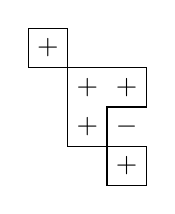
\begin{tikzpicture}[x=0.5cm,y=0.5cm]
\draw (0,3) rectangle (1,4);
\draw (1,3) -- (3,3) -- (3,2) -- (2,2) -- (2,1) -- (1,1) -- cycle;
\draw (2,0) rectangle (3,1);
\node at (0.5,3.5) {$+$};
\node at (1.5,2.5) {$+$};
\node at (2.5,2.5) {$+$};
\node at (1.5,1.5) {$+$};
\node at (2.5,1.5) {$-$};
\node at (2.5,0.5) {$+$};
\end{tikzpicture}
\end{adjustbox}
\end{center}

Легко проверить, что в 2-мерном случае
\begin{equation}
Z(\beta)=\sum_{\text{контурам}}(\lambda)^L;
\tag{5}
\end{equation}
где
\begin{equation*}
\lambda=e^{-2\beta};\qquad L\text{ --- длина контура}
\end{equation*}

Далее, можно записать (из (5))
\begin{equation}
Z(\beta)=\prod_x\int d\psi^1(x)\,d\psi^2(x)\,d\psi^3(x)\,d\psi^4(x)\,\exp\{A[\psi]\},
\tag{6}
\end{equation}
[Под всеми четырьмя $\psi$ зачеркнуты нижние индексы:
\Unclear{GELFAND-P001524}{equation-06-cancelled-subscripts}{$x$?; либо $1,2,3,4$?}.]

где
$\psi^\alpha$ --- грассмановы переменные (по 4 на любом узле);

[Слева над формулой (7) отдельная помета:
\Unclear{GELFAND-P001524}{margin-equation-07}{$x$? / $z$?}.]
\begin{equation}
A[\psi]= -\frac{1}{2}\sum_{x,\alpha}(\psi(x)\,C\,\psi(x))
+\lambda\sum_{x,\alpha}\psi(x+\alpha)P_\alpha\psi(x)
\tag{7}
\end{equation}
\begin{equation}
(\psi C\psi)=\psi^\alpha C^{\alpha\beta}\psi^\beta;
\tag{8}
\end{equation}
$C^{\alpha\beta}$ --- определенная матрица
(надлежащего определения)
% Resolved after independent original/crop review: bbox (1190,2110,1600,2265), 3x.

\noindent (9) $C=$
\SourceFigure{GELFAND-P001524}{matrix-09}{Схематическая матрица в квадратных скобках: видны два нуля, последовательно смещенные вниз и вправо от верхнего левого угла, небольшой диагональный точечный след, нуль в нижнем правом углу, $+1$ в верхней правой части и $-1$ в нижней левой. Расположение и смысл незаполненных мест требуют сверки с оригиналом.}

В непрерывном пределе
\begin{equation}
C\longleftrightarrow\gamma^5=\hat\sigma_1\hat\sigma_2
\tag{10}
\end{equation}
$\sigma_j$ --- матрицы Паули
\begin{equation}
P_\alpha=\frac{1+\vec\alpha\,\vec\sigma}{2}\quad\text{--- проектор}
\tag{11}
\end{equation}

Контуры сводятся к направленным блужданиям.
При блуждании возникает множитель $\lambda e^{i\Delta\varphi/2}$, к-рый

\SourcePage{GELFAND-P001525}{38}
% Review bbox original px (left,top,right,bottom): top 275,45,1830,545; enlargement 3x.
% Review bbox original px (left,top,right,bottom): label 2160,55,2280,170; enlargement 5x.
% Review bbox original px (left,top,right,bottom): equation-12-left 85,555,1610,835; enlargement 3x.
% Review bbox original px (left,top,right,bottom): equation-12-right 1640,565,2240,940; enlargement 3x.
% Review bbox original px (left,top,right,bottom): equation-13 80,1090,1150,1260; enlargement 3x.
% Review bbox original px (left,top,right,bottom): parafermions 320,1320,1900,1660; enlargement 3x.
% Review bbox original px (left,top,right,bottom): equation-14 140,1870,1320,2070; enlargement 3x.
% Review bbox original px (left,top,right,bottom): equation-15 120,2070,2190,2350; enlargement 3x.
% Review bbox original px (left,top,right,bottom): bottom 80,2600,2150,3375; enlargement 3x.
% Review bbox original px (left,top,right,bottom): feynman-words 325,415,1390,530; enlargement 4x.
% Review bbox original px (left,top,right,bottom): diagram-lower 335,840,1115,1110; enlargement 4x.
% Review bbox original px (left,top,right,bottom): eq13-differential 775,1105,925,1235; enlargement 10x.
% Review bbox original px (left,top,right,bottom): eq14-cancel 735,1900,965,2060; enlargement 10x.
% Review bbox original px (left,top,right,bottom): epsilon-middle 615,2970,855,3070; enlargement 8x.
% Review bbox original px (left,top,right,bottom): specific-heat-plot 265,2270,655,2600; enlargement 4x.
% Review bbox original px (left,top,right,bottom): remark 280,1700,2070,1855; enlargement 3x.
% Review bbox original px (left,top,right,bottom): lower-path-label 535,1000,635,1095; enlargement 10x.
% Page label reviewed at bbox (2160,55,2280,170), 5x; final digit has two closed lobes.
входит в амплитуду (комплексная вероятность);
$\Delta\varphi$ --- угол поворота.

$e^{i\Delta\varphi/2}$ --- факторы Каца--Уорда

Объяснение задачи блуждания --- Фейнман.
% Resolved after independent original/crop review: bbox (720,415,960,530), 4x.

\begin{equation}
\begin{aligned}
\sum_{\mathcal P_{x_1,x_2}}\prod\lambda e^{i\Delta\varphi/2}
&=\langle\psi^\alpha(x_1)\psi^\beta(x_2)\rangle\\
&=\sum_{\mathcal P_{x_1,x_2}}
\begin{adjustbox}{max width=\linewidth}
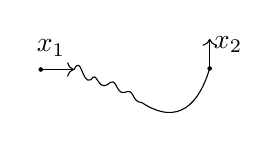
\begin{tikzpicture}[baseline=-0.8ex,x=0.65cm,y=0.65cm]
\fill (0,0) circle (0.045);
\node at (0.2,0.42) {$x_1$};
\draw[->] (0,0) -- (0.65,0);
\draw (0.65,0) .. controls (0.8,0.3) and (0.8,-0.3) .. (0.98,-0.2)
.. controls (1.1,0) and (1.1,-0.4) .. (1.3,-0.3)
.. controls (1.5,-0.1) and (1.45,-0.48) .. (1.63,-0.45)
.. controls (1.85,-0.35) and (1.75,-0.63) .. (1.98,-0.65)
.. controls (2.7,-1.12) and (3.1,-0.65) .. (3.3,0.02);
\fill (3.3,0.02) circle (0.045);
\draw[->] (3.3,0.02) -- (3.3,0.6);
\node at (3.66,0.48) {$x_2$};
\end{tikzpicture}
\end{adjustbox}\\
&=W^{\alpha\beta}(x_1,x_2)
\end{aligned}
\tag{12}
\end{equation}

\begin{equation*}
\mathcal P_{x_1,x_2}=\{\text{пути от }x_1\text{ к }x_2\}
\end{equation*}
\SourceFigure{GELFAND-P001525}{path-under-definition}{Повторный рисунок пути от $x_1$ слева к $x_2$ справа: от левой отмеченной точки направлена горизонтальная стрелка вправо; далее идет волнистая линия с несколькими подъемами и спусками, затем изгиб вверх к правой отмеченной точке, от которой стрелка направлена вверх. Под первой стрелкой имеется мелкая неуверенно читаемая подпись или угловая помета.}

По определению:
\begin{equation}
\int d\psi=0,\qquad
\int\Unclear{GELFAND-P001525}{equation-13-overwriting}{d\psi}\cdot\psi=1
\tag{13}
\end{equation}

Парафермионные переменные бывают нужны
(см. Фатеев В.; Замолодчиков А. ЖЭТФ, 1985).
[Под строкой: конструктивно постр. в конформной теор. поля.]

\underline{Замечание}. Вычисление теплоемкости в предст. (6)

Положим
\begin{equation}
F(\beta)=\ln Z(\beta)
\tag{14}
\end{equation}
[Между знаком равенства и $\ln Z(\beta)$ зачеркнута запись:
\Unclear{GELFAND-P001525}{equation-14-cancelled-factor}{$-T$? / $-1/\beta$?}.]

\begin{equation}
\frac{d^2F(\beta)}{d\beta^2}\sim\frac{Z''}{Z}-\frac{(Z')^2}{Z^2}
=\underset{\text{Теплоемкость}}{\underline{\underline{C(\beta)}}}
\sim(\beta-\beta_c)^{-\alpha}
\tag{15}
\end{equation}

% Plot reviewed at bbox (265,2270,655,2600), 4x. Left-pointing horizontal arrow is retained.
\begin{center}
\begin{adjustbox}{max width=\linewidth}
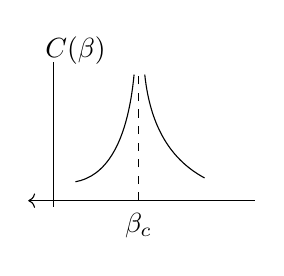
\begin{tikzpicture}[x=0.8cm,y=0.8cm]
\draw[<-] (-0.4,0) -- (3.2,0);
\draw (0,-0.1) -- (0,2.2);
\node at (0.35,2.38) {$C(\beta)$};
\draw[dashed] (1.35,0) -- (1.35,2.1);
\node at (1.35,-0.4) {$\beta_c$};
\draw (0.35,0.3) .. controls (0.8,0.38) and (1.17,0.85) .. (1.28,2.0);
\draw (1.45,2.0) .. controls (1.54,1.15) and (1.88,0.64) .. (2.4,0.36);
\end{tikzpicture}
\end{adjustbox}
\end{center}

Показатель $\alpha$ --- критический индекс. Имеем:
\begin{equation}
C(\beta)=\sum_x\langle\varepsilon(x)\varepsilon(0)\rangle
=\Unclear{GELFAND-P001525}{equation-16-unsummed-expression}{\frac{1}{|x|^{2\Delta_\varepsilon}}},
\tag{16}
\end{equation}
где
\begin{equation*}
\varepsilon=(\psi\,\Unclear{GELFAND-P001525}{energy-bilinear-symbol}{\rho}\,\psi)
\end{equation*}
Здесь
$\Delta_\varepsilon$ однозначно связано с $\alpha$ и называется
\underline{аномальной размерностью}:
[Последние два слова подчеркнуты волнистой линией.]

\SourcePage{GELFAND-P001526}{unlabelled}
% Review bbox original px (left,top,right,bottom): 1526-eq17 90,85,1000,310; enlargement 3x.
% Review bbox original px (left,top,right,bottom): 1526-topwords 1060,100,1840,285; enlargement 3x.
% Review bbox original px (left,top,right,bottom): 1526-topparenthesis 290,320,1500,445; enlargement 3x.
% Review bbox original px (left,top,right,bottom): 1526-thirdcase 300,485,950,625; enlargement 3x.
% Review bbox original px (left,top,right,bottom): 1526-eq18 80,645,1530,925; enlargement 3x.
% Review bbox original px (left,top,right,bottom): 1526-eq19 85,925,2050,1200; enlargement 3x.
% Review bbox original px (left,top,right,bottom): 1526-eq20 90,1220,1180,1460; enlargement 3x.
% Review bbox original px (left,top,right,bottom): 1526-sdefinition 285,1480,1500,1775; enlargement 3x.
% Review bbox original px (left,top,right,bottom): 1526-psi 345,1790,1580,1995; enlargement 3x.
% Review bbox original px (left,top,right,bottom): 1526-indices 330,2020,1120,2400; enlargement 3x.
% Review bbox original px (left,top,right,bottom): 1526-eq21 90,2400,830,2660; enlargement 3x.
% Review bbox original px (left,top,right,bottom): 1526-eq22 80,2650,1540,2925; enlargement 3x.
% Review bbox original px (left,top,right,bottom): 1526-diagram 1510,2660,2020,3210; enlargement 3x.
% Review bbox original px (left,top,right,bottom): 1526-topordinary 335,330,650,430; enlargement 5x.
% Review bbox original px (left,top,right,bottom): 1526-scaling 625,327,1030,435; enlargement 5x.
% Review bbox original px (left,top,right,bottom): 1526-eq19first 800,950,1065,1095; enlargement 8x.
% Review bbox original px (left,top,right,bottom): 1526-eq19second 1270,955,1725,1090; enlargement 5x.
% Review bbox original px (left,top,right,bottom): 1526-mindices 1680,1010,1940,1130; enlargement 8x.
% Review bbox original px (left,top,right,bottom): 1526-sparenthesisfirst 345,1645,650,1760; enlargement 5x.
% Review bbox original px (left,top,right,bottom): 1526-sparenthesisrest 630,1640,1130,1760; enlargement 4x.
% Review bbox original px (left,top,right,bottom): 1526-grassmann 765,1860,1510,1975; enlargement 4x.
% Review bbox original px (left,top,right,bottom): 1526-flagindices 407,2050,740,2160; enlargement 6x.
% Review bbox original px (left,top,right,bottom): 1526-cubeface 730,2230,1000,2400; enlargement 5x.
% Review bbox original px (left,top,right,bottom): 1526-pre21 325,2395,680,2495; enlargement 5x.
% Review bbox original px (left,top,right,bottom): 1526-between21-22 230,2590,420,2675; enlargement 8x.
% Review bbox original px (left,top,right,bottom): 1526-diagramcaption1 1580,2880,1940,3080; enlargement 4x.
% Review bbox original px (left,top,right,bottom): 1526-diagramcaption2 1640,3030,2010,3210; enlargement 4x.
% Review bbox original px (left,top,right,bottom): 1526-beta18 425,680,575,850; enlargement 8x.
% Review bbox original px (left,top,right,bottom): 1526-epsilon17 815,90,920,300; enlargement 8x.
% Review bbox original px (left,top,right,bottom): 1526-eq22-epsilon 800,2670,1270,2860; enlargement 3x.
% Review bbox original px (left,top,right,bottom): 1526-cancelled19 982,940,1065,1055; enlargement 10x.
% Review bbox original px (left,top,right,bottom): 1526-sparenthesisfirst10 370,1665,610,1755; enlargement 10x.
% Original image 2408 x 3480; full frame reviewed. Reproducible review crop bboxes use original pixels (left,top,right,bottom).
% P001526: eq17 (90,85,1000,310) 3x; d definition (1060,100,1840,285) 3x; scaling parenthesis (290,320,1500,445) 3x, (335,330,650,430) 5x, (625,327,1030,435) 5x; heading (300,485,950,625) 3x.
\begin{equation}
\alpha=\frac{d-2\Delta_{\varepsilon}}{d-\Delta_{\varepsilon}},\qquad d\text{ --- размерность пр-ва}
\tag{17}
\end{equation}
(обычное скейлинговое соотношение)

\underline{3-мерный случай.}

% P001526: eq18 (80,645,1530,925) 3x; beta (425,680,575,850) 8x; epsilon subscripts (815,90,920,300) 8x.
\begin{equation}
Z(\beta)=\prod_{\text{ребрам}}\int d\psi^{\alpha}_{x,\mu}\,\exp\{A[\psi]\}
\tag{18}
\end{equation}

% P001526: eq19 (85,925,2050,1200) 3x; first term (800,950,1065,1095) 8x; quartic superscripts (1270,955,1725,1090) 5x; final M indices (1680,1010,1940,1130) 8x; overdrawn psi exponent (982,940,1065,1055) 10x.
\begin{equation}
A[\psi]=\frac{1}{2}\sum_{\text{ребрам}}
\left(\psi^{\alpha}C^{\alpha\beta}\psi^{\Unclear{GELFAND-P001526}{eq19-psi-index}{\beta}}\right)
+\lambda\sum_{\text{граням}}
\left(\psi^{\alpha}\psi^{\beta}\psi^{\gamma}\psi^{\delta}M_{\alpha\beta,\Unclear{GELFAND-P001526}{eq19-m-indices}{\gamma\delta\text{ / }\delta\gamma}}\right)
\tag{19}
\end{equation}
[В первом слагаемом верхний индекс последнего $\psi$ и закрывающая скобка густо обведены.]

% P001526: eq20 (90,1220,1180,1460) 3x; surface definition (285,1480,1500,1775) 3x; parenthesis (345,1645,650,1760) 5x, (630,1640,1130,1760) 4x, (370,1665,610,1755) 10x.
\begin{equation}
Z(\beta)=\sum_{S}\lambda^{A(S)},
\tag{20}
\end{equation}
где $S$ --- замкн. поверхность в $R^3$,

(\Unclear{GELFAND-P001526}{surface-parenthesis}{скруч. / окруж.} разные роды)

% P001526: Grassmann variables (345,1790,1580,1995) 3x, (765,1860,1510,1975) 4x; flag and labels (330,2020,1120,2400) 3x, (407,2050,740,2160) 6x, (730,2230,1000,2400) 5x.
$\psi^{\alpha}_{x,\mu}$ --- грассмановы переменные

\begin{center}
\begin{adjustbox}{max width=\linewidth}
\begin{tikzpicture}
\node (flag-x) at (0,0) {$x$};
\node at (0.6,0) {$\subset$};
\node (flag-alpha) at (1.2,0) {$\alpha$};
\node at (1.8,0) {$\subset$};
\node (flag-mu) at (2.4,0) {$\mu$};
\node at (4,0) {--- \underline{флаг}};
\node (flag-edge) at (0.8,-1.2) {ребро};
\node (flag-face) at (3,-1.2) {грань кубика};
\draw (flag-alpha) -- (flag-edge);
\draw (flag-mu) -- (flag-face);
\end{tikzpicture}
\end{adjustbox}
\end{center}

% P001526: word before eq21 (325,2395,680,2495) 5x; eq21 (90,2400,830,2660) 3x; connector (230,2590,420,2675) 8x.
Посчитаем
\begin{equation}
\ln Z=F,
\tag{21}
\end{equation}
тогда
% P001526: eq22 (80,2650,1540,2925) 3x; correlator (800,2670,1270,2860) 3x; diagram with caption (1510,2660,2020,3210) 3x, caption (1580,2880,1940,3080) 4x, (1640,3030,2010,3210) 4x.
\begin{equation}
F''=\sum\langle\varepsilon(x)\varepsilon(0)\rangle=\sum
\tag{22}
\end{equation}
\SourceFigure{GELFAND-P001526}{eq22-surface-diagram}{После последнего знака суммы нарисованы два небольших квадратных окончания с подписями $x$ слева и $0$ справа; окончания соединены верхней и нижней дугами. Между дугами расположен вертикальный овал: его правая часть густо обведена, левая состоит из отдельных штрихов. Характер утолщений у верхней и нижней точек овала не вполне различим.}
(рождение замкнутой фермионной струны)

\SourcePage{GELFAND-P001527}{39}
% Review bbox original px (left,top,right,bottom): 1527-line1 265,40,1725,190; enlargement 3x.
% Review bbox original px (left,top,right,bottom): 1527-line2 270,220,1820,360; enlargement 3x.
% Review bbox original px (left,top,right,bottom): 1527-line3 270,335,2010,465; enlargement 3x.
% Review bbox original px (left,top,right,bottom): 1527-line4 275,435,1430,570; enlargement 3x.
% Review bbox original px (left,top,right,bottom): 1527-label 2170,45,2290,160; enlargement 3x.
% Review bbox original px (left,top,right,bottom): 1527-noncontinuous 1200,55,1370,165; enlargement 8x.
% Review bbox original px (left,top,right,bottom): 1527-cancelword 405,418,670,505; enlargement 8x.
% Review bbox original px (left,top,right,bottom): 1527-cancelglyph 1380,345,1460,475; enlargement 10x.
% Review bbox original px (left,top,right,bottom): 1527-datecorrection 1045,452,1160,555; enlargement 8x.
% Review bbox original px (left,top,right,bottom): 1527-cancelglyph-full 1315,330,1425,470; enlargement 10x.
% Original image 2408 x 3480; all content is in the upper strip, the remainder is blank. Full frame reviewed.
% P001527: first sentence (265,40,1725,190) 3x; abbreviation (1200,55,1370,165) 8x; bibliography authors (270,220,1820,360) 3x; title (270,335,2010,465) 3x; volume/year (275,435,1430,570) 3x; page label (2170,45,2290,160) 3x.
Дальше надо реш. задачу в непр. пределе.

\underline{Лит-ра}: Доценко, Поляков ($\sim60$ стр.)

(в кн. Advanced Studies in Pure
[зачёркнутый знак: \Unclear{GELFAND-P001527}{bibliography-cancelled-sign}{\&}]
Mathematics,

% P001527: strongly cancelled text (405,418,670,505) 8x; cancelled sign (1315,330,1425,470) 10x; retraced first year digit (1045,452,1160,555) 8x.
[Ниже «в кн.» зачёркнуто:
\Incomplete{GELFAND-P001527}{bibliography-cancelled-word}{Короткий фрагмент, густо зачёркнутый несколькими горизонтальными и обводящими штрихами; полностью прочитать первоначальные буквы не удалось.}]

v. 16, 1988)
[Первая цифра года густо обведена.]



\end{document}
